\chapter{Decidability}\label{ch-12}

In this chapter, the nature and limitations of algorithms are
explored. We will first look at the general properties that can be
ascertained about finite automata and FAD languages. For example,
we might like to be able to enter the state transition table of a
DFA into a suitably sized array and then run a program that determines
whether the DFA was connected. An algorithm for checking this
property was outlined in Chapter \ref{ch-3}. Similarly, we have seen that
it is possible to write a program to check whether an arbitrary DFA
is minimal. We know this property can be reliably checked because
we proved that the algorithms in Chapter 3 could be applied to
ascertain the correct answer for virtually every conceivable DFA.
There are an infinite number of DFAs about which the question can
be posed, and yet our algorithm decides the question correctly in
all cases. In the following section we consider questions that can
be asked about more complex languages and machines.

%
% Do not forget to fix up all references to sections and chapters using
% label and ref (this is important for the index).
%

In the latter part of this chapter, we will see that unlike the questions in
Sections \ref{sec-12.1} and \ref{sec-12.2}, there are some questions that are in
a fundamental sense unanswerable in the general case. That is, there cannot
exist an algorithm that correctly answers such a question in all cases. These
questions will be called undecidable. An undecidable question about Pascal
programs is considered in detail in Section \ref{sec-12.3} and is independent of
advanced machine theory. The concept of undecidability is addressed formally in
Section \ref{sec-12.4}, and other undecidable problems are also presented.

% 12.1 DECIDABLE QUESTIONS ABOUT REGULAR LANGUAGES
\section{Decidable Questions About Regular Languages}\label{sec-12.1}

Recall that a procedure is a finite set of instructions that
unambiguously specifies deterministic, discrete steps for performing
some task. In this chapter, the task will generally involve providing
the correct answer to some yes-no question. Most questions that
involve a numerical answer can be rephrased as a yes-no question
of similar complexity. For example, the question ``What is the minimum
number of states necessary for a DFA to accept the language represented
by the regular expression $R$?'' has the yes-no analog ``Does there
exist a DFA with fewer than, say, five states that accepts the
language represented by the regular expression $R$?'' Clearly, if we
can answer the first question, the second question is easy to answer.
Conversely, if questions like the second one can be answered for
any number we wish (rather than just five), then the answer to the
first question can be deduced.

Recall also that an \Index{algorithm} is a procedure that is guaranteed to halt in all
instances. Note that ``guaranteed to halt'' does not mean that there is a fixed
time limit on how long it may take to finish the procedure for all inputs; some
instances may take far longer than others. For example, the question ``Does
there exist a DFA with fewer than ten states that accepts the language
represented by $\pmb{ab}(\pmb{b}\cup\pmb{c})^*$?'' will probably take less time
to answer than ``Does there exist a DFA with fewer than ten states that accepts
the language represented by $\pmb{a}^*\pmb{b}((\pmb{b}^*\pmb{d}\cup\pmb{c}^*
\pmb{b})\pmb{d}\cup\pmb{e})^*?$''

It is important to keep in mind that algorithms are intended to provide a
general solution to a vast array of similar problems and are (usually) not
limited to a single specific instance. As an example, consider the task of
sorting a file containing the three names:
\begin{quote}
Williams \\
Jones \\
Smith
\end{quote}
A variety of sorting algorithms, when applied to this file, will produce the
correct output. It is also possible to write a program that ignores its input
and always prints the lines
\begin{quote}
Jones \\
Smith \\
Williams
\end{quote}
This program does yield the correct answer for the particular problem we wished
to solve, and indeed it solves the sorting problem for all files that contain
exactly these three particular names in some arbitrary order (there are six such
files). Thus, this trivial program is an algorithm that solves the sorting
problem for these six specific instances. A slightly more complex program might
be capable of printing two or three distinct answers, depending on the input,
and thus solve the sorting problem for an even larger (but still finite) class
of instances.

It should be clear that producing an algorithm that solves a finite set of
instances is no great accomplishment, since these algorithms are guaranteed to
exist. Such an algorithm could be programmed as one big case statement, which
identifies the particular input instance and produces the corresponding output
for that instance. Algorithms that apply to an infinite set of instances are of
much more theoretical and practical interest.

% Definition 12.1
\begin{dfn}\label{dfn-12.1}\index{instance of a question}
Given a set of \emph{instances} and a yes-no \emph{question} that can be
applied to those instances, we will say that the question is
\emph{\Index{decidable}} if there is an algorithm for determining in each
instance the (correct) answer to the question.
\end{dfn}

A more precise definition of decidability is presented in Section \ref{sec-12.4}, based
on the perceived relationship between Turing machines and algorithms. As
mentioned earlier, if the set of instances is finite, an algorithm is guaranteed
to exist, no matter how complex the question appears to be.

\subsection*{Example 12.1}\label{ex-12.1}

A typical set of instances might be the set of all deterministic finite
automata over a given alphabet $\Sigma$; a typical question might be whether a
given automaton accepts at least one string in $\Sigma^*$.

It is possible to devise an algorithm to correctly answer the question posed
in Example \ref{ex-12.1} for every finite automaton $A=\langle\Sigma,S,s_0,\delta,F\rangle$.
The first idea that might come to mind is to simply look at strings from
$\Sigma^*$ in an orderly manner and use $\DBAR$ to determine whether that string
is accepted by $A$; if we find a string that does reach a final state, it is
clear that the answer to the question should be ``YES$-L(A)\not=\emptyset$,''
while if we never find a string that is accepted, the answer should be ``NO$-
L(A)=\emptyset$.'' This procedure is guaranteed to halt and give the correct
answer if the language is indeed nonempty. However, the procedure will never
halt and answer NO (in a finite amount of time) because there are an infinite
number of strings in $\Sigma^*$ that must be checked. A modification of this
basic idea is necessary to produce a procedure that will halt under all
circumstances (that is, to produce an algorithm ).

% Theorem 12.1
\begin{thm}\label{thm-12.1}
Given any alphabet $\Sigma$ and a DFA $A=\langle\Sigma,S,s_0,\delta,F\rangle$,
it is decidable whether $L(A)=\emptyset$.

\emph{Proof.} Let $n=\|S\|$. Since both $\Sigma$ and $S$ are finite sets,
\[ B = \{\lambda\}\cup\Sigma\cup\Sigma^2\cup\cdots\cup\Sigma^{n-1} \]
is a finite set, and we can examine each string of this set and still have a
procedure that halts. There is clearly an algorithm for determining the set $C$
of all states that are reached by these few strings. Specifically,
\[ C=\{\DBAR(s_0,x)\ |\ x\in\Sigma^*\wedge |x|<n\}=\{\DBAR(s_0,x)|x\in B\}. \]
Note that Theorem \ref{thm-2.7} implies that if a string (of \emph{any} length) is
accepted by $A$ then there is another string of length less than $n$ that is
also accepted by $A$. Consequently, it is sufficient to examine only the
``short'' strings contained in $B$ rather than examine all of $\Sigma^*$. If any
of the strings in $B$ lead to a final state (that is, if $C\cap F\not=\emptyset$),
then the answer to the question is clearly ``NO$-L(A)$ is \emph{not} empty,''
while if $C\cap F=\emptyset$, then Theorem \ref{thm-2.7} guarantees that ``YES$-L(A)$
\emph{is} empty'' is the correct answer. We have therefore constructed an
algorithm (which computes $C$ and then examines $C\cap F$, both of which can be
done in a finite amount of time) for determining whether the language accepted
by a given machine is empty.
\end{thm}

The definition of $C$ does not suggest the most efficient algorithm for
calculating the set $C$; better strategies are available. The technique is
similar to that employed to find the state equivalence relation $E_A$. $C$ is
actually the set of connected states $S^c$, which can be calculated recursively
as indicated in Definition \ref{dfn-3.10}. Note that Theorem \ref{thm-12.1} answers the question
posed in Example \ref{ex-12.1}. The set of instances to which this question applies can
easily be expanded. It can be shown that it is decidable whether $L(A)=\emptyset$
for any NDFA $A$ by first employing Definition \ref{dfn-4.5} to find the equivalent DFA
$A^d$ and then applying the method outlined in Theorem \ref{thm-12.1} to that machine. It
is possible to find a much more efficient algorithm for answering this question
that does not rely on the conversion to a DFA (see the exercises).

Just as the algorithm for converting an NDFA into a DFA allows the emptiness
question to be answered for NDFAs, the techniques in Chapter 6 justify that
the similar question for regular expressions is decidable. That is, since
every regular expression has an equivalent DFA, the question of whether a
regular expression describes any strings is clearly decidable. Similar
extensions can be applied to most of the results in this section. Just as we can
decide whether a DFA $A$ accepts any strings, we can also decide if $A$ accepts
an infinity of strings, as shown by Theorem \ref{thm-12.2}. This can be proved by a
related appeal to Theorem \ref{thm-12.1}, but an efficient algorithm for answering this
question depends on the following lemma.

% Lemma 12.1
\begin{lmm}\label{lmm-12.1}
Let $\Sigma$ be an alphabet, $A=\langle\Sigma,S,s_0,\delta,F\rangle$ be a finite
automaton, $n=\|S\|$, and $M=\{x\ |\ x\in L(A)\wedge |x|\geq n\}$. Then, if $M\not=
\emptyset$, $M$ must contain a string of minimal length (call it $x_m$), and
furthermore $|x_m| < 2n$.

\emph{Proof.} The proof is obtained by repeated application of the pumping lemma
with $i=0$ (see the exercises and Theorem \ref{thm-2.7}).
\end{lmm}

A question similar to the one posed in Theorem \ref{thm-12.1} is ``Does a given DFA
accept a finite or an infinite number of strings?'' This is also a decidable
question, as demonstrated by the following theorem. The proof is based on the
observation that a DFA $A$ that accepts no strings of length greater than some
fixed constant must by definition recognize a finite set, while the pumping
lemma implies that if $L(A)$ contains a sufficiently long string, then $L(A)$
must contain an infinite number of related strings.

% Theorem 12.2
\begin{thm}\label{thm-12.2}
Given any alphabet $\Sigma$ and a DFA $A=\langle\Sigma,S,s_0,\delta,F\rangle$,
it is decidable whether $L(A)$ is an infinite set.

\emph{Proof.} Let $n=\|S\|$. Clearly, if $A$ accepts no strings of length $n$ or
greater, then L(A) is finite. From the pumping lemma, we know that if $A$
accepts even one string of length equal to or greater than $n$, then $A$ must
accept an infinite number of strings. We still cannot check all the strings of
length greater than $n$ and have a procedure that halts, so Lemma \ref{lmm-12.1} will be
invoked to argue that if a long string is accepted by $A$, then a string whose
length is in the range $n\leq |x| < 2n$ must be accepted, and it is therefore
sufficient to check the strings in this limited range. Thus, our algorithm will
consist of computing the intersection of $\{\delta(s_0,y)\ |\ y\in\Sigma^*\wedge n
\leq |y| < 2n\}$ and $F$. $L(A)$ is infinite iff this intersection is
nonempty.
\end{thm}

If we were to write a program that consulted the matrix containing the state
transition table for $A$ to actually determine $\{\delta(s_0,y)\ |\ y\in\Sigma^*
\wedge n\leq |y| < 2n\}$, it would be very inefficient to implement this
computation as implied by the definition. Repeatedly looking up entries in the
state transition table to determine \DBAR\ for each word in this large class of
specified strings would involve an enormous duplication of effort. It is far
better to recursively calculate $R_i=\{\DBAR(s_0,x)\ |\ x\in \Sigma^i\}$, which
represents the set of all states that can be reached by strings of length
exactly $i$. This can be easily computed by defining $R_0=\{s_0\}$ and using the
recursive formula
\[ R_{i+1}= R_i \cup \{\delta(s,\pmb{a})\ |\ \pmb{a}\in\Sigma,s\in R_i\} \]
Successive sets can thereby be calculated from $R_0$. When $R_i$ is reached, it
is checked against $F$, and the algorithm halts and returns Yes if they have a
common state. Otherwise, $R_{n+1}$ through $R_{2n-1}$ are checked, and No is
returned if no final state appears in these groups. This method is easily
adaptable to nondeterministic finite automata by setting $R_0$ to be the set of
all start states and adjusting the definition of $R_{i+1}$ to conform to NDFA
notation.

The involved arguments presented in Lemma \ref{lmm-12.1} and the proof of
Theorem \ref{thm-12.2} are necessary to justify that the above efficient
recursive algorithm correctly answers the question of whether a finite automaton
accepts an infinite number of strings. However, if we were simply interested in
justifying that it is decidable whether $L(A)$ is infinite, without worrying about efficiency, it would have been
much more convenient to simply adapt the result of Theorem \ref{thm-12.1}. In
particular, we could have easily built a DFA that accepts all strings of length
at least $n$, form the ``intersection'' machine, and apply Theorem \ref{thm-12.1} to the new machine.

Specifically, if $A$ is an $n$-state deterministic finite automaton, consider
the DFA $A_n=\langle\Sigma,\{r_0,r_1,r_2,\ldots,\\r_n\},r_0,\delta_{\!n},\{r_n\}
\rangle$, where $\delta_{\!\!n}$ is defined by
\[ (\forall i=0,1,\ldots,n)(\forall\pmb{a}\in\Sigma)(\delta_{\!\!n}(r_i,\pmb{a})=
	r_{\text{max}\{i+1,n\}}) \]
It is easy to show that $L(A_n)=\{x\in\Sigma^*|\ \ |x|\geq n\}$, and building
$A^{\cap}$ as specified in Lemma \ref{lmm-5.1} produces a DFA for which $L(A^{\cap})=\{x
\in L(A)\ |\ \ |x|\geq n\}$. The question of whether $L(A)$ is infinite now becomes
the question of whether $L(A^{\cap})$ is nonempty, which was shown to be
decidable by Theorem \ref{thm-12.1}.

An indication of the nature of the automaton $A_{n}$ is given in Figure
\ref{fig-12.1}. The above argument provides a much shorter and clearer proof of
Theorem \ref{thm-12.2}, but it should not be construed to be the basis of an efficient
algorithm. Forming the intersection of $A$ and $A_{n}$ involves well over
$n^2$ states, and thus applying the technique described in Theorem \ref{thm-12.1} to
$A^{\cap}$ may involve more than $n^2$ iterations. For our purposes, we will
henceforth be content to discover whether various tasks are merely possible and
not be concerned with efficiency.

% Figure 12.1
\begin{figure}[tbh]
\centerline{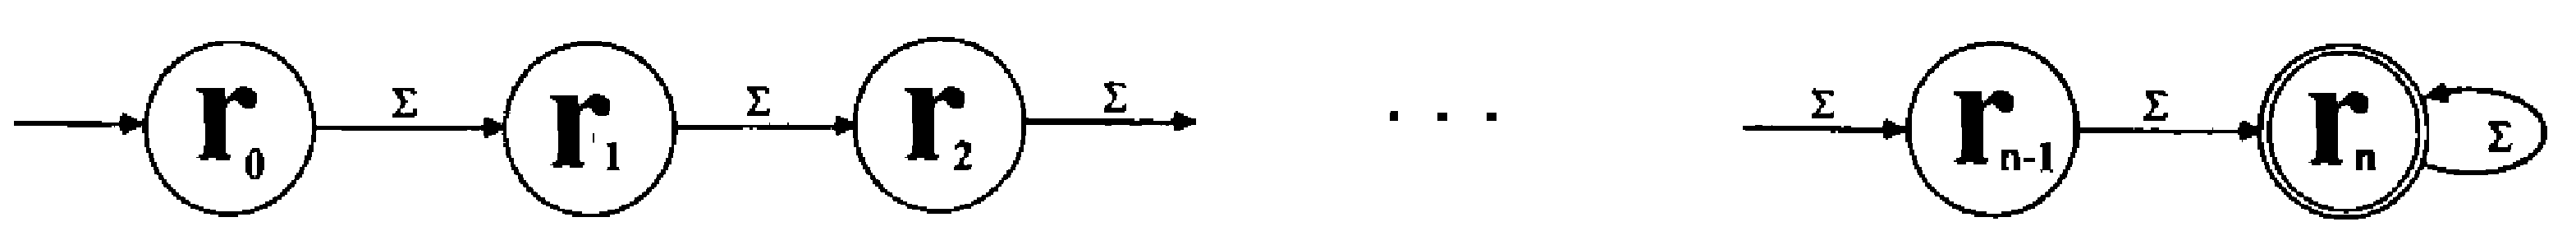
\epsfig{figure=ToFAfigures/fig12-1.eps,width=6in}}
\caption{The automaton $A_n$}\label{fig-12.1}
\end{figure}

The following theorem answers a major question about DFAs: ``Are two
given deterministic finite automata equivalent?'' At first glance,
this appears to be a hard question; an initial strategy might be
to check longer and longer strings, and answer ``No, they are not
equivalent'' if a string is found that is accepted by one machine
but is not accepted by the other. As in the proof of Theorems \ref{thm-12.1}
and \ref{thm-12.2}, we would again be faced with the task of determining when
we could confidently stop checking strings and answer ``Yes, they
are equivalent.''

Such a strategy can be made to work, but an easier method is again
available.  We are essentially checking whether the start state of
the first machine treats strings differently than does the start
state of the second machine. This problem was addressed in Chapter
\ref{ch-3}, and an algorithm that accomplished this sort of checking has
already been presented. This observation provides the basis for the
proof of the following theorem.

% Theorem 12.3
\begin{thm}\label{thm-12.3}
Given any alphabet $\Sigma$ and two DFAs $A_1=\langle\Sigma,S_1,s_{0_1},\delta_1,
F_1\rangle$ and $A_2=\langle\Sigma,S_2,s_{0_2},\delta_2,F_2\rangle$, it is
decidable whether $L(A_1)=L(A_2)$.

\emph{Proof.} Without loss of generality, assume that $S_1\cap S_2=\emptyset$,
and construct a new DFA defined by $A=\langle\Sigma,S_1\cup S_2,s_{0_1},\delta,
F_1\cup F_2\rangle$, where
\begin{center}\begin{tabular}{r@{ = }l}
$(\forall s\in S_1\cup S_2)(\forall\pmb{a}\in\Sigma)\delta(s,\pmb{a})$ &
	$\left\{\begin{tabular}{l@{$\qquad$}l}
		$\delta_1(s,\pmb{a})$, & iff \  $s\in S_1$ \\
		$\delta_2(s,\pmb{a})$, & iff \  $s\in S_2$
		\end{tabular}
	\right.$
\end{tabular}\end{center}
Corollary \ref{cor-3.5} outlines the algorithm for constructing $E_A$ for this machine,
and it should be clear from the definition of $A$ that $s_{0_1}E_As_{0_2}
\Leftrightarrow L(A_1)=L(A_2)$.
\end{thm}

\subsection*{Example 12.2}\label{ex-12.2}

Consider the two machines $A_1$ and $A_2$ displayed in Figure \ref{fig-12.2}. The machine
$A$ constructed according to Theorem \ref{thm-12.3} would look like the diagram inside the
dotted box shown in Figure \ref{fig-12.3}. This new machine is very definitely
disconnected, and in this example $s_{0_1}$ is not related to $s_{0_2}$ by $E_A$ since
these two states treat $\pmb{ab}$ differently ($\pmb{ab}$ is accepted by $A_1$
and rejected by $A_2$). The reader is encouraged to generate another example
using two equivalent machines, and verify that the two original start states
would indeed be related by $E_A$.

% Figure 12.2
\begin{figure}[tbh]
\centerline{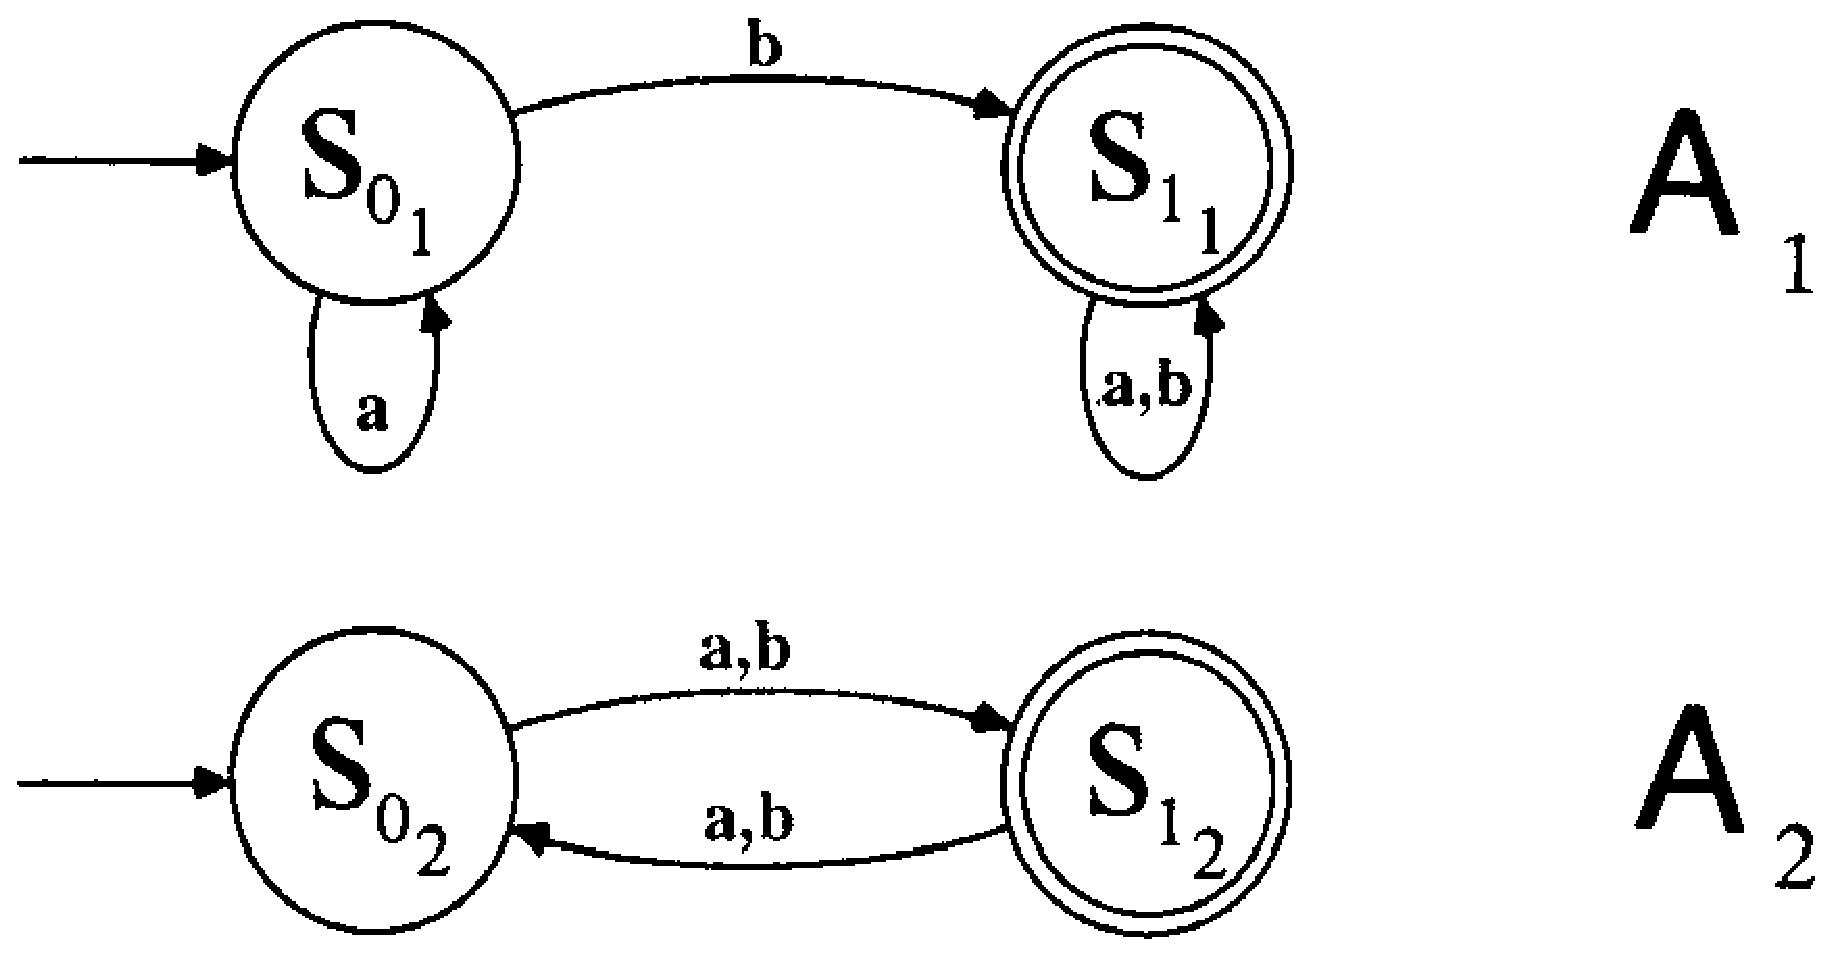
\epsfig{figure=ToFAfigures/fig12-2.eps,width=3.5in}}
%The field \ref{ex-12.2} resolves to '12.1" for some reason...
%\caption{The DFAs discussion in Example \ref{ex-12.2}}\label{fig-12.2}
\caption{The DFAs discussion in Example 12.2}\label{fig-12.2}
\end{figure}

% Figure 12.3
\begin{figure}[tbh]
\centerline{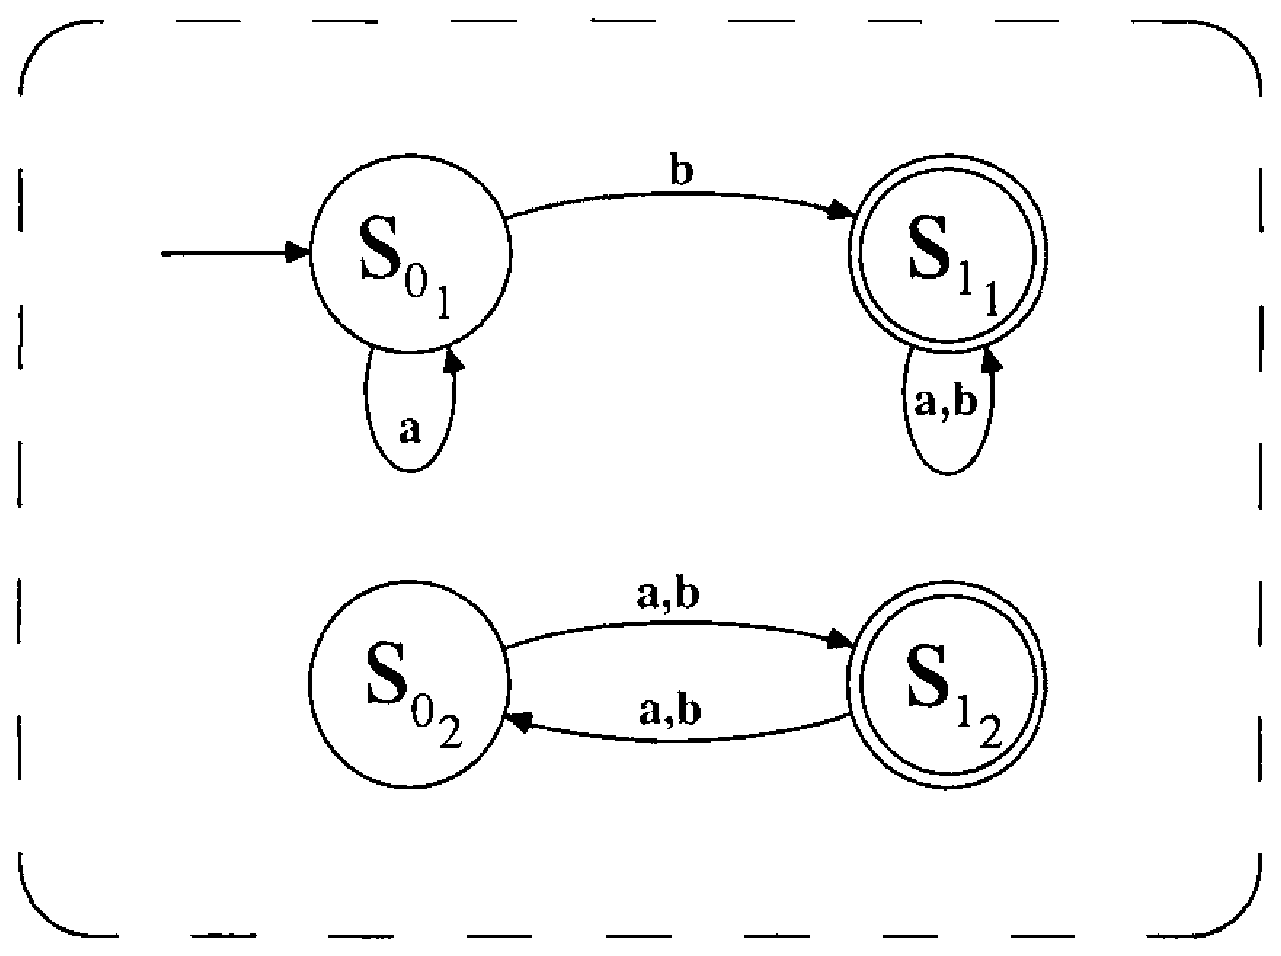
\epsfig{figure=ToFAfigures/fig12-3.eps,width=3.5in}}
%The field \ref{ex-12.2} resolves to '12.1" for some reason...
%\caption{The composite DFA discussed in \ref{ex-12.2}}\label{fig-12.3}
\caption{The composite DFA discussed in Example 12.2}\label{fig-12.3}
\end{figure}

The following theorem explores the relationship between the complexity of a
given regular expression and the size of the corresponding minimal DFA.

% Theorem 12.4
\begin{thm}\label{thm-12.4}
Given any alphabet $\Sigma$ and a regular expression $R$ over $\Sigma$, it is
decidable whether there exists a DFA with fewer than five final states that
accepts the language described by $R$.

\emph{Proof.} Given $R$, Lemma \ref{lmm-6.2} indicates the algorithm (generated
by the constructions presented in Theorems \ref{thm-5.2}, \ref{thm-5.4}, and
\ref{thm-5.5}) for building some NDFA that accepts the regular set corresponding
to $R$. Definition \ref{dfn-4.5} outlines the algorithm for converting this NDFA
into a DFA. Theorem \ref{thm-3.7} and Corollary \ref{cor-3.5} indicate the
algorithms for minimizing this DFA. Counting the number of final states in this
minimal machine will allow the question to be answered correctly.
\end{thm}

The careful reader may have noticed that the minimal machine described in
Chapters \ref{ch-2} and \ref{ch-3} was only advertised to have the minimum
\emph{total} number of states and has not yet been guaranteed to have the smallest
number of \emph{final} states (perhaps there is an equivalent machine with many
more nonfinal states but fewer final states). An investigation of the
relationship between the final states of the minimal machine and the equivalence
classes comprising the right congruence generated by this language will show
that no equivalent DFA can have fewer final states than the minimal machine
has (see the exercises).

The proofs of Theorems \ref{thm-12.3} and \ref{thm-12.4} are good examples of
using existing algorithms to build new algorithms. This technique should be
applied whenever possible in the following exercises. It is certainly useful in
resolving the following question about grammars.

Given two right linear grammars $G_1=\langle\Omega_1,\Sigma,S_1,P_1\rangle$ and
$G_2=\langle\Omega_2,\Sigma,S_2,P_2\rangle$, it is clearly \emph{decidable}
whether $G_2$ is equivalent to $G_1$. An algorithm can be formed that simply:
\begin{enumerate}
\item Uses the construction presented in Lemma \ref{lmm-8.2} to find $A_{G_1}$
	and $A_{G_2}$.
\item Converts these NDFAs to two DFAs called $A_1$ and $A_2$.
\item Appeals to the algorithm presented in Theorem \ref{thm-12.3} to correctly
answer the question.
\end{enumerate}
A trivial extension of this idea proves the following theorem.

% Theorem 12.5
\begin{thm}\label{thm-12.5}
It is decidable whether two given regular grammars $G_1=\langle\Omega_1,\Sigma,
S_1,P_1\rangle$ and $G_2=\langle\Omega_2,\Sigma,S_2,P_2\rangle$ are equivalent.

\emph{Proof.} See the exercises.
\end{thm}

Most of the decidability questions we have asked about languages recognized
by finite automata or described by regular expressions can also be answered
for languages generated by grammars through a similar transformation of existing
algorithms. Such algorithms are generally not the most efficient ones available,
and it can often be instructive to develop a new method from scratch. This is
especially true of the following question, which has no analog in the realms of
finite automata or regular expressions.

% Theorem 12.6
\begin{thm}\label{thm-12.6}
It is decidable whether a given right-linear grammar $G=\langle\Omega,\Sigma,S,
P\rangle$ contains any useless nonterminals.

\emph{Proof.} Recall that a nonterminal is \emph{useless} if it can never appear
in the derivation of any valid terminal string. Essentially, only two things can
prevent a nonterminal $X$ from being effectively used somewhere in a valid
derivation: either $X$ can never appear as part of a partial derivation that
begins with only the start symbol (no matter how many productions we apply), or,
once $X$ is generated, it can never lead to a valid \emph{terminal} string.

Finding the members of $\Omega$ that can be produced from $S$ is a simple
recursive procedure: Begin with $Z_0=\{S\}$ and form $Z_1$ by adding to $Z_0$
all the nonterminals that appear on the right side of productions that are used
to replace $S$. Then form $Z_2$ by adding to $Z_1$ all the nonterminals that
appear on the right side of productions that are used to replace members of $Z_1$
and so on. More formally:
\[ Z_0 = \{S\} \]
and for $i \geq 1$,
\[ Z_{i+1} = Z_i\cup\{Y\in\Omega\ |\ (\exists x\in\Sigma^*)(\exists T\in Z_i)\ni T
	\rightarrow xY\text{ is a production in }P\} \]
Clearly, $Z_0\subseteq Z_1\subseteq\cdots\subseteq Z_n\subseteq\cdots\subseteq
\Omega$, and as was shown for similar collections of nested entities (such as
$E_{0A},E_{1A},\ldots$ in Chapter \ref{ch-3}), after a finite number of steps we
will reach the point where $Z_m=Z_{m+1}$ and $Z_m$ will then represent the set
of \emph{all} nonterminals that can be reached from the start symbol $S$.

In a similar fashion, we can generate another nested sequence of sets $W_0,W_1,
\ldots,$ where $W_i$ represents the set of all nonterminals that can produce
a \emph{terminal} string in $i$ or fewer steps. We are again guaranteed to reach
a point where $W_n=W_{n+i}$ and $W_n$ will indeed be the set of all nonterminals
that can \emph{ever} produce a valid terminal string.

$Z_m\cap W_n$ is thus the set of all \emph{\Index{useful}} members of $\Omega$, and
$\Omega -(Z_m\cap W_n)$ is therefore the set of all \Index{useless} nonterminals.
\end{thm}

\subsection*{Example 12.3}\label{ex-12.3}

$G_4=\langle\{S,A,B,C,V,W,X\},\{\pmb{a},\pmb{b},\pmb{c}\},S,\{S\rightarrow\pmb{a
b}A|\pmb{bb}B|\pmb{cc}V,A\rightarrow\pmb{b}C|\pmb{c}X,B\rightarrow\pmb{ab},
C\rightarrow\lambda|\pmb{c}S,V\rightarrow\pmb{a}V|\pmb{c}X,W\rightarrow\pmb{aa}|
\pmb{a}W,X\rightarrow\pmb{b}V|\pmb{aa}X\}\rangle$ contains three useless
nonterminals, $V$, $W$, and $X$. Recursively calculating the sets described in
the above proof yields:
\begin{center}\begin{tabular}{l@{$\quad$}l}
$Z_0=\{S\}$ & $W_0=\{\ \ \}$ \\
$Z_1=\{S,A,B,V\}$ & $W_1=\{C,B,W\}$ \\ 
$Z_2=\{S,A,B,V,C,X\}$ & $W_2=\{C,B,W,A,S\}$ \\ 
$Z_3=\{S,A,B,V,C,X\}$ & $W_3=\{C,B,W,A,S\}$
\end{tabular}\end{center}
Thus $W$ cannot be generated from the start symbol, and $V$ and $X$ cannot
produce terminal strings. The \emph{useful} symbols are $Z_2\cap W_2=\{S,A,B,C\}$,

The techniques employed here should look somewhat familiar. They involve
iteration methods similar to those developed in Chapter \ref{ch-3}. In fact, it
is possible to apply the connectivity algorithms for nondeterministic finite
automata to this problem by transforming the right-linear grammar $G$ into the
NDFA $A_G$, as defined in the proof of Lemma \ref{lmm-8.2}. The automaton
corresponding to the grammar in Example \ref{ex-12.3} is shown in Figure
\ref{fig-12.4}. Note that the state labeled $\<W\>$ is inaccessible, which
means that it cannot be reached from $\<S\>$. This indicates that there is no
sequence of productions starting with the start symbol $S$ that will produce
a string containing $W$.

Checking whether a nonterminal such as $V$ can produce a terminal string is
tantamount to checking whether the language accepted by $A^V_G$ is nonempty,
where $A^V_G$ is $A_G$ with the start state moved to the state labeled $\<V\>$.
Since both $L(A^V_G)$ and $L(A^X_G)$ are empty, $V$ and $X$ are useless.

\section{Other Decidable Questions}\label{sec-12.2}

It is fairly easy to find succinct algorithms that answer most of the reasonable
questions one might ask about representations of regular languages. For each of
the more complex classes of languages, there are many reasonable questions that
are not decidable. Several of these will be presented in the following sections.
In this section, we consider some of the answerable questions that can be asked
about the more robust machines and grammars.

% Theorem 12.7
\begin{thm}\label{thm-12.7}
Given any context-free grammar $G$, it is decidable whether $L(G)=\emptyset$.

\emph{Proof.} In Theorem 9.3, a scheme was presented that specified how to build
several automata that would be used to identify the useless nonterminals in
$G=\langle\Sigma,\Gamma,S,P\rangle$. Since $L(G)=\emptyset$ iff the start symbol
$S$ is useless, there is an algorithm for testing whether $L(G)=\emptyset$.
\end{thm}

It is also possible to tell whether a context-free grammar generates a finite
or an infinite number of distinct words. The proof is based on the same
principle that was employed in the pumping theorem proof: the presence of long
strings implies that some useful nonterminal $A$ must derive a nontrivial
sentential form containing $A$. The start state $S$ must produce a useful
sentential form containing $A$, and $A$ can then be used to generate an infinite
series of distinct strings.

% Figure 12.4
\begin{figure}
\centerline{\epsfig{figure=ToFAfigures/fig12-4.eps,height=7in}}
\caption{The automaton discussed in Example 12.3}\label{fig-12.4}
\end{figure}

% Theorem 12.8
\begin{thm}\label{thm-12.8}
Given any context-free grammar $G$, it is decidable whether $L(G)$ is infinite.

\emph{Proof.} Let $G=\langle\Sigma,\Gamma,S,P\rangle$ be a context-free grammar.
By Theorem 9.5, there exists a Chomsky normal form grammar $G'=\langle\Sigma,
\Gamma',S,P'\rangle$ that is equivalent to $G$. Let $n=2^{|\Gamma'|}$. By
Theorem \ref{thm-9.7}, any string in $L(G)$ of length $n$ or greater can be
pumped and will imply that $L(G)$ is infinite. An argument similar to that of
Lemma \ref{lmm-12.1} will show that it is sufficient to check strings in the
set $\{y\ |\ y\in\Sigma^*\wedge n\leq |y| < 2n\}$ for membership in $L(G)$. There
are only a finite number of derivation sequences that can produce words in this
range. The algorithm for determining whether $L(G)$ is infinite will check
whether
\[ \{y\ |\ y\in L(G)\wedge n\leq |y| < 2n\} \]
is empty; if so, $L(G)$ is finite, and $L(G)$ is infinite otherwise.
\end{thm}

The exercises explore more efficient methods for searching for a string that
can be pumped. The intimate correspondence between context-free grammars and
pushdown automata guarantees that similar questions about PDAs are decidable.

% Corollary 12.1
\begin{cor}\label{cor-12.1}
Given any pushdown automaton $P$, it is decidable whether:
\begin{enumerate}[{\bf a.}]
\item $L(P)$ is empty.
\item $L(P)$ is finite.
\item $L(P)$ is infinite.
\end{enumerate}

\emph{Proof.} By Theorem \ref{thm-10.3}, every PDA $P$ has a corresponding
context-free grammar $G_P$. The algorithms described in Theorems \ref{thm-12.7}
and \ref{thm-12.8} can be applied to $G_P$ to determine the nature of $L(G_P)$,
and since $L(P)=L(G_P)$, the same questions about $P$ are likewise decidable.
\end{cor}

Given a particular word $x$ and a context-free grammar $G$, it is decidable
whether $x$ can be generated by $G$. In fact, this question can be decided for
context-sensitive grammars, too. The proof heavily relies on the fact that no
sentential form longer than $x$ can possibly generate $x$ in the absence of
contracting productions in the grammar.

% Theorem 12.9
\begin{thm}\label{thm-12.9}
Given any context-sensitive grammar $G$ and any word $x$, it is decidable
whether $x\in L(G)$.

\emph{Proof.} Let $G=\langle\Sigma,\Gamma,S,P\rangle$ be a context-sensitive
grammar and let $x\in\Sigma^n$ (for an arbitrary $n$). It is possible to construct a (finite) graph and
apply existing algorithms from graph theory to answer the question of whether
$G$ generates $x$. The nodes of the graph will correspond to the strings from
$(\Sigma\cup\Gamma)^*$ of length $n$ or less. The (directed) edges from a node
representing a given sentential form $w$ lead to the strings (of length $n$ or
less) that can be generated from $w$ by applying a single production from $P$.
Both the sentential form $x$ and $S$ will appear in this graph, and the question
of whether $x\in L(G)$ is equivalent to the question of whether there is a path
from $S$ to $x$. There are many standard algorithms for determining paths and
components in a graph, and thus the question of whether $x\in L(G)$ is decidable.
\end{thm}

The generation of all the edges in the graph generally involves more effort
than is needed to answer the question. A more efficient method is similar to
the recursive calculations used to find the set of connected states in a DFA.
Beginning with $\{S\}$, the production set $P$ can be consulted to determine the
labels of nodes that can be derived from $S$ in one step. These new labels can
be added to the set of accessible sentential forms, and the added nodes can be
checked until no new labels are found. The set of sentential forms will then 
consist of
\[ \{w\in(\Sigma\cup\Gamma)^*|\ S\ \DRightarrow w \wedge |w|\leq n\} \]
and contain all words in $L(G)$ of length $\leq n$, If we are only interested in
the specific word $x$, then the algorithm can return Yes as soon as $x$ appears
in the set of accessible sentential forms and would return No if $x$ did not
appear by the time the set stopped growing.

The above algorithm will suffice for any grammar that does not contain
contracting productions, but can clearly give the wrong answers when applied to
type 0 grammars. Since the length of sentential forms can both grow and shrink
in unrestricted grammars, the word $x$ may actually be generated by a sequence
of productions that at some point generates a sentential form longer than $x$.
Such a sequence would not be considered by the method outlined in Theorem
\ref{thm-12.9}, and the algorithm might answer No when the correct answer is Yes.
We could define a procedure that looked at larger and larger graphs (consisting
of more and longer sentential forms), which would halt and answer Yes if a
derivation sequence for $x$ was discovered. If $x$ actually can be generated by
$G$, this method will eventually uncover the appropriate sequence. We therefore
have a procedure that will reliably tell us if a word can be generated by an
unrestricted grammar. Unless we include a specification of when to stop and
answer No, this procedure is not an algorithm. In later sections, we will see
that it is \emph{impossible} to determine, for an arbitrary type 0 grammar $G$,
if an arbitrary word $x$ is not generated by $G$. The question of whether $x\in
L(G)$ is not decidable for arbitrary grammars.

It turns out that there are many reasonable questions such as this one that
cannot be determined algorithmically. We begin our overview of undecidable
problems with an analysis of a very reasonable question concerning Pascal
programs. Subsequent sections consider undecidable questions concerning the
grammars and machines covered in this text.

\section{An Undecidable Problem}\label{sec-12.3}\index{undecidable problems}

Having now developed a false sense of security about our ability to produce
algorithms for determining many properties about machines and languages, we
now step back and see whether there is anything we cannot do algorithmically. A
simple counting argument will show that there are too many things to calculate
and not enough algorithms with which to calculate them all. It may be helpful to
review the section on cardinality in Chapter \ref{ch-0} and recall that there
are different orders of infinity. A diagonalization argument showed that the
natural numbers could not be put in one-to-one correspondence with the real
numbers; there are simply too many real numbers to allow such a matching to
occur. A similar mismatch occurs when comparing the (countable) number of
algorithms to the (uncountable) number of possible yes-no functions.

By definition, an algorithm is a \emph{finite} list of instructions, written
over some finite character set. As such, there are only a countable number of
different algorithms that can be written. It may be helpful to consider the set
of all Pascal programs and view each file that contains the ASCII code for a
program, which is essentially a sequence of zeros and ones, as one very long
binary integer. Clearly, an infinite number of Pascal programs can be written,
but no more programs than there are binary integers, so the number of such files
is indeed countable.

Now consider the possible lists of answers that could be given to questions
involving a countable number of instances. We will argue that there are an
uncountable number of yes-no patterns that might describe the answers to such
questions. Notice that the descriptions for automata, grammars, and the like
are also finite, and thus there are a countable number of DFAs, a countable
number of grammars, and so on, that can be described. The questions we asked in
the previous sections were therefore applied to a countable number of instances,
and these instances could be ordered in some well-defined way, much as the
natural numbers are ordered. If we think of a yes response corresponding to the
digit 1 and a no response corresponding to 0, then the corresponding series of
answers to a particular question can be thought of as an unending sequence of
0s and 1s. By placing a decimal point at the beginning of the sequence, each
such pattern can be thought of as a binary fraction, representing a real number
between $.00000\ldots=0$ and $.111111\ldots=1$. Conversely, each such real
number in this range represents a sequence of yes-no answers to some question.
Since there are an uncountable number of real numbers between 0 and 1, there are
an uncountable number of answers that might be of interest to us. Some of these
answers cannot be obtained by algorithms, since there are not enough algorithms
to go around. Thus, there must be many questions that are not decidable.

It is not immediately apparent that the existence of undecidable questions is
much of a drawback; perhaps all the ``interesting'' questions are decidable.
After all, there are an uncountable number of real numbers, yet all computers
and many humans seem to make do with just the countable number of rational
numbers. Unfortunately, there are many simple and meaningful questions that are
undecidable. We discuss one such question now; others are considered in the next
section.

Just about every programmer has had the experience of running a program that
never produces any output and never shows any sign of halting. For programs
that are fairly short, this is usually not a problem. For major projects that
are expected to take a very long time, there comes an agonizing moment when we
have to give up hope that it is on the verge of producing a useful answer and
stop the program on the assumption that it has entered an infinite loop. While
it would be very nice to have a utility that would look over a program and
predict how long it would run, most of us would settle for a device that would
simply predict whether or not it will ever halt.

It's a good bet that you have never used such a device, which may at first seem
strange since a solution to the \emph\Index{halting problem} would certainly provide
information that would often be useful. If you have never thought about this
before, you might surmise that the scarcity of such programs is a consequence of
any one of several limiting factors. Perhaps they are inordinately expensive to
run, or no one has taken the time to implement an existing scheme, or perhaps no
one has yet figured out how to develop the appropriate algorithms. In actuality,
no one is even looking for a ``halting'' algorithm, since no such algorithm can
possibly exist.

\index{undecidable problems!Pascal halting problem|(}Let us consider the implications that would arise if such an algorithm could be
programmed in, say, Pascal. We can consider such an algorithm to be implemented
as a Boolean function called HALT, which looks at whatever program happens to
be in the file named data.p and returns the value TRUE if that program will
halt, and returns FALSE if the program in data.p would never halt. Perhaps this
function is general enough to look at source code for many different languages,
but we will see that it is impossible for it to simply respond correctly even
when looking solely at Pascal programs.

The programmer of the function HALT would likely have envisioned it to be used
in a program such as CHECK, shown in Figure \ref{fig-12.5}. We will use it in a
slightly different way and show that a contradiction arises if HALT really did
solve the halting problem. Our specific assumptions are that:
\begin{enumerate}
\item HALT is written in Pascal.
\item HALT always gives a correct answer to the halting problem, which means:
\begin{enumerate}
\item It always returns an answer after a finite amount of time.
\item The answer returned is FALSE if the Pascal program in data.p would never
halt.
\item The answer returned is TRUE if the Pascal program in data.p would halt (or
if the program in data.p will not compile).
\end{enumerate}
\end{enumerate}

Consider the program TEST in Figure \ref{fig-12.6}, which is structured so that
it will run forever if the function HALT indicates that the program in the file
data.p would halt, and simply quits if HALT indicates that the program in data.p
would not halt. Some interesting things happen if we run this program after
putting a copy of the source code for TEST in data.p.

If HALT does not produce an answer, then HALT certainly does not behave as
advertised, and we have an immediate contradiction. HALT is supposed to be an
algorithm, so it must eventually return with an answer. Since HALT is a Boolean
function, we have only two other cases to consider.

% Figure 12.5
\begin{figure}
{\tt
\begin{tabbing}
abc\=abc\=end \kill
program CHECK; \\
\{ envisioned usage of HALT \} \\
\> function HALT:boolean; \\
\> begin \\
\>\> \{ marvelous code goes here \} \\
\> end \{ HALT \} \\
\\
begin \{ CHECK \} \\
if HALT then \\
\> writeln('The program in file data.p will halt') \\
else \\
\> writeln('The program in file data.p will not halt') \\
end \{ CHECK \}.
\end{tabbing}
}
\caption{A possible usage of HALT}\label{fig-12.5}
\end{figure}

{\bf Case 1}: HALT returns a value of TRUE to the calling program TEST. This has
two consequences, the first of which is implied by the asserted behavior of HALT.
\begin{enumerate}[i.]
\item If halt does what it is supposed to do, this means that the program in
data.p halts. We ran this program with the source code for TEST in data.p, so
TEST must actually halt.
\end{enumerate}
The second consequence comes from examining the code for TEST, and noting
what happens when HALT returns TRUE.
\begin{enumerate}[i.]
\addtocounter{enumi}{1}
\item The {\tt if} statement in the program TEST then causes the infinite loop
to be entered, and TEST runs forever, doing nothing particularly useful.
\end{enumerate}
Our two consequences are that TEST halts and TEST does not halt. This is a
clear contradiction, and so case 1 never occurs.

{\bf Case 2}: HALT returns a value of FALSE to the calling program TEST. This
likewise has two consequences. Considering the advertised behavior of HALT, this
must mean that the program in data.p, TEST, must not halt. However, the code for
TEST shows that if HALT returns FALSE we execute the else statement, write one
line, and then stop. TEST therefore halts. TEST must again both halt and not
halt.

Whichever way we turn, we reach a contradiction. The only possible conclusion
is that the function HALT does not behave as advertised. It must either return
no answer, or give an incorrect answer.

It should be clear that the problem cannot be fixed by having the programmer who
proposed the function HALT fiddle with the code; the above contradiction will be
reached regardless of what code appears between the {\tt begin} and {\tt end}
statements in the function HALT. We have shown that any such proposed function
is guaranteed to behave inappropriately when fed a program such as TEST. In
actuality, there are an infinite number of programs that cause HALT to misbehave,
but it was sufficient to demonstrate just one failure to justify that no such
function can solve the general problem.

% Figure 12.6
\begin{figure}
{\tt
\begin{tabbing}
abc\=abc\=end\kill
program TEST; \\
\{ to be placed in the file data.p \} \\
var FOREVER: boolean; \\
\> function HALT: boolean; \\
\> begin \\
\>\> \{ marvelous code goes here \} \\
\> end; \{ HALT \} \\
\\
begin \{ TEST \} \\
FOREVER := false; \\
if HALT then \\
\> repeat \\
\>\> FOREVER := false; \\
\> until FOREVER \\
else \\
\> writeln('This program halts') \\
end \{ TEST \}.
\end{tabbing}
}.
\caption{Another program incorporating HALT}\label{fig-12.6}
\end{figure}

\index{halting problem!in Pascal}
The above argument demonstrates that the \emph{halting problem} for
Pascal programs is \emph{\Index{undecidable}} or \emph{\Index{unsolvable}}. That
is, there does not exist a Pascal program that can always decide correctly, when
fed an arbitrary Pascal program, whether that program halts.

If we were to define an algorithm as ``something that can be programmed in
Pascal,'' we would have shown that there is no algorithm for deciding whether
an arbitrary Pascal program halts. One might suspect that this is therefore not
a very satisfying definition of what an algorithm is, since we have a concise,
well-stated problem that cannot be solved using Pascal. It is generally agreed
that the problem does not lie with some overlooked feature that was
inadvertently not incorporated into Pascal. Clearly, all programming languages
suffer from similar inadequacies. For example, an argument similar to the one
presented for Pascal would show that no C program can be devised that can tell
which C programs can halt. Thus, no other programming language can provide a
more robust definition of what an algorithm is.

\index{halting problem!in C}\index{undecidable problems!C halting problem}
There are variations on this theme that likewise lead to contradictions. Might
there be a Pascal program that can check which C programs can halt? If you
believe that every Pascal program can be rewritten as an equivalent C program,
the answer is definitely no; a Pascal program that checks C programs could then
be rewritten as a C program (which checks C programs), and we again reach a
contradiction.\index{undecidable problems!Pascal halting problem|)}

It is generally agreed that the limitations do not arise from some correctable
inadequacy in our current methods of implementing algorithms. That is, the
limitations of algorithmic solutions seem to be inherent in the nature of
algorithms. Programming languages, Turing machines, grammars, and all other
proposed systems for implementing algorithms have been shown to be subject to
the same limitations in computational power. The use of Turing machines to
implement algorithms has several implications that apply to the theory of
languages. These are explored in the following sections.

\section{Turing Decidability}\label{sec-12.4}\index{Turing machine!undecidable problems}

In the previous section, we saw that no Pascal program could always correctly
predict when another Pascal program would halt. A similar statement was true
for C programs, and Turing machines, considered as computing devices, are no
different; no Turing machine solves the halting problem.

Each of us is probably familiar with the way in which a Pascal program reads a
file, and hence it is not hard to imagine a Pascal program that reacts to the
code for another Pascal program. As long as the input alphabet contains at least
two symbols, encodings can be defined for the structure of a Turing machine,
which allows the blueprint for its finite state control to be placed on the
input tape of another Turing machine. A binary encoding\index{Turing machine!encoding} might be given for the
number of states, followed by codes that enumerate the moves from each of the
states. Just as we are not presently concerned about the exact ASCII codes that
define the individual characters in a file containing a Pascal program, we need
not be concerned with the specific representation used to encode a Turing
machine on an input tape.

Consider input tapes that contain the encoding of a Turing machine, followed
by some delimiter, followed by an input word. Assume there exists a Turing
machine $H$ that, given such an encoding of an arbitrary machine and an input word,
always correctly predicts whether the Turing machine represented by that
encoding halts for that particular word. This assumption leads to a
contradiction exactly as shown in the last section for Pascal programs. We would
be able to use the machine $H$ as a submachine in another Turing machine that
halts exactly when it is not supposed to halt, and thereby show that $H$ cannot
possibly behave properly.

% Theorem 12.10
\begin{thm}\label{thm-12.10}\index{undecidable problems!Turing machine halting problems|(}
Given a Turing machine $M$ and a word $w$, it is undecidable whether $M$ halts
when the string $w$ is placed on the input tape.

\emph{Proof.} The proof is essentially the same argument that was presented in
the last section.
\end{thm}

We will see that the unsolvability of the halting problem will imply that it
is not decidable whether a given string will cause a Turing machine to halt and
print $\pmb{Y}$. If a word is accepted, this fact can eventually be discovered,
but we cannot reliably tell which words are rejected by an arbitrary Turing
machine. If we could, we would have an algorithm for computing the complement of
any Turing-acceptable language. In the next section, we will show that there are
Turing-acceptable languages that have complements that are not Turing-acceptable,
which means that a general algorithm for computing complements cannot exist.

A problem equivalent to the halting problem involves the question of whether
an arbitrary type 0 grammar accepts a given word. This can be seen to be almost
the same question as was asked of Turing machines.

% Theorem 12.11
\begin{thm}\label{thm-12.11}
Given a type 0 grammar $G$ and a word $w$, it is undecidable whether $G$
generates $w$.

\emph{Proof.} If this question were decidable, it would provide an algorithm for
solving the halting problem, which is known to be undecidable. That is, if there
existed an algorithm for deciding whether $w\in L(G)$, there would also be an
algorithm for deciding whether $w$ is accepted by a Turing machine. The Turing
machine algorithm would operate as follows:

Given an arbitrary Turing machine $M$, modify $M$ to produce $M'$, an equivalent
machine that halts only when it accepts. Use Definition 11.8 to find the
corresponding type 0 grammar $G_{M'}$, which is also equivalent to $M$. The
algorithm that predicts whether $w\in L(G_{M'})$ can now be used to decide
whether $M$ halts on input $w$.

This scheme would therefore solve the halting problem for an arbitrary Turing
machine, and hence the algorithm that predicts whether $w\in L(G)$ cannot exist.
Thus, $w\in L(G)$ is undecidable for arbitrary type 0 grammars.
\end{thm}

Given the intimate correspondence between Turing machines and type 0 grammars,
it is perhaps not surprising that it is just as hard to solve the membership
question for type 0 grammars as it was to solve the halting problem for Turing
machines. We now consider a question that may initially appear to be more
tractable than the halting problem. However, it will be shown to be unsolvable
by the same reasoning used in the last theorem: if this question could be
decided, then the halting problem would be decidable.

% Theorem 12.12
\begin{thm}\label{thm-12.12}
Given an arbitrary Turing machine $T$, it is undecidable whether $T$ accepts
$\lambda$.

\emph{Proof.} Assume that there exists an algorithm for deciding whether $T$
accepts $\lambda$. That is, assume that there exists a Turing machine $X$ that,
when fed an encoding of any Turing machine $T$, halts with $\pmb{Y}$ when $T$
would accept $\lambda$ and halts with $\pmb{N}$ whenever $T$ rejects $\lambda$.
$X$ can then be used to determine whether an arbitrary Turing machine $M$ would
accept an arbitrary word $x$. Given a machine $M$ and a string $x$, it is easy
to modify $M$ to produce a new Turing machine $T_{M_x}$, which accepts $\lambda$
exactly when $M$ accepts $x$. $T_{M_x}$, is formed by adding a new start state
that checks whether the read head is initially scanning a blank (that is, if
$\lambda$ is on the input tape). If not, control remains in this state, and
$T_{M_x}$ never halts. However, if the initially scanned symbol is a blank, new
states are used to write $x$ on the input tape and return the read head to the
leftmost symbol of $x$. Control then passes to the original start state of $M$.
In this manner, $T_{M_x}$ accepts $\lambda$ exactly when $M$ accepts $x$.

This correspondence makes it possible to use the Turing machine $X$ as a
submachine in another Turing machine $X_H$ that solves the halting problem. That
is, given an input tape with an encoding of a machine $M$ followed by the
symbols for a word $x$, $X_H$ can be easily programmed to modify the encoding of
$M$ to produce the encoding of $T_{M_x}$ and leave this new encoding on the
input tape before passing control to the submachine $X$. $X_H $then accepts
exactly when $T_{M_x}$ accepts $\lambda$, which happens exactly when the original machine $M$ halts
on input $x$. $X_H$ would therefore represent an algorithm for solving the
halting problem, which we know cannot exist. The portion of the machine that
modifies the encoding of $M$ is quite elementary, so it must be the submachine
$X$ that cannot exist. Thus, there is no algorithm that can accomplish the task
for which $X$ was designed, that is, determining whether an arbitrary Turing
machine $T$ accepts the empty string.
\end{thm}

The conclusion that $X$ was the portion of $X_H$ that behaves improperly is akin
to the observation in the previous section that the main part of the Pascal
program TEST was valid, and hence it must be the function HALT that behaves
incorrectly.\index{undecidable problems!Turing machine halting problems|)}

\section{Turing-Decidable Languages}\label{sec-12.5}

We now consider languages whose criteria for membership is related to the
halting problem. Define the language $D$ to be those words that either are not
encodings of Turing machines or are encodings of machines that would halt with
$\pmb{Y}$ when presented with their own encoding on their input tape. The
language $D$ is Turing acceptable, since a multitape machine\index{multi-tape Turing machine}\index{Turing machine!multi-tape} could copy the
input word to a second tape, check whether the encoding truly represented a
valid Turing machine, and then use the ``directions'' on the second tape to
simulate the action of the encoded machine on the original input. The multitape
machine would halt with $\pmb{Y}$ if the encoding was invalid or if the
simulated machine ever accepts.

On the other hand, the complement of $D$ is not Turing acceptable. Let $U$ be
the set of all valid encodings of Turing machines that do \emph{not} halt when
fed their own encodings. Then $U=\ \sim\!\!D$, and there does not exist a
machine $T$ for which $L(T)=U$. If such a machine existed, it would have an
encoding, and this leads to the same problem encountered with the HALT function
in Pascal. This encoding of $T$ is either a word in $U$ or is not a word in $U$;
both cases lead to contradictions. If the encoding of $T$ belongs to $U$, then
by definition of $U$ it does not halt when fed its own encoding. But the
assumption that $L(T)=U$ requires that $T$ halt with $\pmb{Y}$ for all encodings
belonging to $U$, which means $T$ must halt when fed its own encoding. A similar
contradiction is also reached if the encoding of $T$ does not belong to $U$.
Therefore, no such Turing machine $T$ can exist, and $U$ is an example of a
language that is not Turing-acceptable.

We have finally found a language that is not type 0. A counting argument would
have shown that, since there are only a countable number of type 0 grammars and
an uncountable number of subsets of $\Sigma^*$, there had to be many languages
over $\Sigma$ that are not in \ZSIG\ ( $=\TSIG$). We have now seen that some of these
unrepresentable languages are meaningful sets for which it would be quite
desirable to be able to recognize or generate.

% Theorem 12.13
\begin{thm}\label{thm-12.13}
If $\|\Sigma\|\geq 2$, then \TSIG\ is not closed under complementation.

\emph{Proof.} Encodings of arbitrary Turing machines can be effectively
accomplished with only two distinct symbols in the alphabet. The
Turing-acceptable language $D$ described above has a complement $U$ that is not
Turing-acceptable.
\end{thm}

Our original criteria for belonging to the language $L$ accepted by a Turing
machine $M$ implied that $M$ would eventually halt when presented with any word
in $L$, but we had no guarantees about how $M$ will behave when presented with a
word that is not in $L$. $M$ may halt with $\pmb{N}$ on the tape, or $M$ may run
forever. Indeed, we have just seen a Turing-acceptable language for which this
will be the best we can hope for. Turing machines therefore embody
\emph{procedures}, which are essentially a deterministic set of step-by-step
instructions. We now consider the languages accepted by the subclass of Turing
machines that correspond to \emph{algorithms}, procedures that are guaranteed to
eventually halt under all circumstances.

% Definition 12.2
\begin{dfn}\label{dfn-12.2}\index{H@\HSIG \ (H-sigma )}
Let $\Sigma$ be an alphabet. Define \HSIG\ to be the collection of all
languages that can be recognized by Turing machines that halt on all input.
\end{dfn}

Languages in \HSIG\ are called \emph{\Index{Turing-decidable languages}}\index{language!Turing-decidable}. A
trivial modification shows that $L\in\HSIG$ if there exists a Turing machine
that not only halts upon placing a $\pmb{Y}$ after the input word on an
otherwise blank tape for accepted words, but similarly preserves the input word
and prints $\pmb{N}$ for each rejected string. Such devices will be referred to
as \emph{halting} Turing machines.

% Theorem 12.14
\begin{thm}\label{thm-12.14}
\HSIG\ is closed under complementation.

\emph{Proof.} Let $L$ be a Turing-decidable language. Then there must exist a
Turing machine $H$ for which $L(H)=L$ and that halts with $\pmb{Y}$ or $\pmb{N}$
for all strings in $\Sigma^*$. The finite-state control of $H$ can be easily
modified to produce a Turing machine $H'$ for which $L(H')=\ \sim\!\!L$. All
that is required is to replace every transition in $H$ that prints $\pmb{N}$
with a similar transition that prints $\pmb{Y}$ and likewise make sure that
$\pmb{N}$ will be printed by $H'$ whenever $H$ prints $\pmb{Y}$.
\end{thm}

This result has some immediate consequences.

% Corollary 12.2
\begin{cor}\label{cor-12.2}
There is a language that is Turing acceptable but not Turing decidable. That is,
$\HSIG\subset\TSIG$

\emph{Proof.} Definition \ref{dfn-12.2} implies that $\HSIG\subseteq\TSIG$. By
Theorems \ref{thm-12.13} and \ref{thm-12.14}, these two classes have different
closure properties, and thus they cannot be equal. Therefore, $\HSIG\subset
\TSIG$.
\end{cor}

Actually, we have already seen a language that is Turing acceptable but not
Turing decidable. $D$ was shown to be Turing acceptable, but if $D$ were Turing
decidable, then its complement would be Turing decidable by Theorem
\ref{thm-12.14}. However, $\sim\!\!D=U$, and $U$ is definitely not Turing
decidable since it is not even Turing acceptable.

\OSIG, the context-sensitive languages, is another subclass of \TSIG. It is
possible to determine how \HSIG\ relates to \OSIG\ and thereby insert \HSIG\
into the language hierarchy.

% Corollary 12.3
\begin{cor}\label{cor-12.3}
Every context-sensitive language is Turing decidable. That is, $\OSIG\subseteq
\HSIG$

\emph{Proof.} This is actually a corollary of Theorem \ref{thm-12.9}. Given a
type 1 language $L$, there is a context-sensitive grammar $G$ that generates $L$.
The proof of Theorem \ref{thm-12.9} presented an algorithm for determining
whether an arbitrary word can be generated by $G$. This algorithm can be
implemented as a Turing machine $T_G$ that can determine whether a given word
can be generated by $G$ and always halts with the correct answer. Thus, $L$ is
Turing decidable.
\end{cor}

These implications provide the missing element in the proof of Theorem 11.10, as
stated in the next corollary.

% Corollary 12.4
\begin{cor}\label{cor-12.4}
The class of context-sensitive languages is properly contained in the class of
Turing acceptable languages. That is, $\OSIG\subset\TSIG$.

\emph{Proof.} By the previous corollaries, $\OSIG\subseteq\HSIG$ and $\HSIG
\subset\TSIG$.
\end{cor}

Actually, the context-sensitive languages are properly contained in \HSIG. This
will be shown by exhibiting a language that is recognized by a Turing machine
that halts on all inputs, but that cannot be generated by any context-sensitive
language. The following proof, based on diagonalization, should by now look
familiar.

% Theorem 12.15
\begin{thm}\label{thm-12.15}
Let $\Sigma$ be an alphabet for which $\|\Sigma\|\geq 2$. There is a language
that is Turing decidable but not context sensitive. That is, $\OSIG\subset\HSIG$.

\emph{Proof.} By Corollary \ref{cor-12.3}, $\OSIG\subseteq\HSIG$, and it remains
to be shown that there is a member of \HSIG\ that is not a member of \OSIG. By
the technique described in Theorem \ref{thm-12.9}, every context-sensitive
grammar can be represented by a halting Turing machine, and each such Turing
machine has an encoding of its finite-state control. Define $L$ to be the set of
all encodings of Turing machines that:
\begin{enumerate}
\item Represent context-sensitive grammars.
\item Reject their own encoding.
\end{enumerate}
Providing a scheme for encoding the quadruple for a context-sensitive grammar
is left for the exercises. Any reasonable encoding scheme will make it a simple
task to determine whether a candidate string represents nonsense or a valid
context-sensitive grammar.

$L$ can therefore be recognized by a halting Turing machine that:
\begin{enumerate}
\item Checks if the string on the input tape represents the encoding of a valid
context-sensitive grammar.
\item Calculates the encoding of the corresponding Turing machine.
\item Simulates that Turing machine being fed its own encoding.
\end{enumerate}
This process is guaranteed to halt, since the Turing machine being simulated is
known to be a halting Turing machine. Thus, $L\in\HSIG$. However, if $L\in\OSIG$,
we find ourselves in a familiar dilemma. If there is a context-sensitive grammar
$G_L$ that generates $L$, then this grammar would have a corresponding Turing
machine $T_L$, which would have an encoding $x_L$. If $x_L$ did not belong to
$L$, then by definition of $L$ it would be an encoding of a machine ($T_L$) that
did not reject its own encoding ($x_L$). Thus, $T_L$ recognizes $x_L$, and
therefore the corresponding grammar $G_L$ must generate $X_L$. But then $X_L\in
L(G_L)=L$, contradicting the assumption that $X_L$ did not belong to $L$. If on
the other hand $X_L$ belongs to $L$, then, by definition of $L$, $T_L$ must
reject its own encoding ($x_L$), and thus $x_L\notin L(T_L)=L(G_L)=L$, which is
another contradiction. Thus, no such context-sensitive grammar $G_L$ can exist,
and $L$ is not a context-sensitive language.
\end{thm}

The above diagonalization technique can be generalized; given any enumerable
class $\mathfrak{M}$ of languages whose members are all represented by halting
Turing machines, there must exist a halting Turing machine that recognizes a
language not in $\mathfrak{M}$ (see the exercises). The following theorem
summarizes how the other classes of languages discussed in the text fit in the
language hierarchy.

% Theorem 12.16
\begin{thm}\label{thm-12.16}\index{hierarchy!of language classes}.
Let $\Sigma$ be an alphabet for which $\|\Sigma\|\geq 2$. Then
\[ \DSIG=\WSIG=\RSIG=\GSIG\subset\ASIG\subset\CSIG=\PSIG\subset\LSIG=\OSIG
	\subset\HSIG\subset\ZSIG=\TSIG\subset\wp(\Sigma^*) \]

\emph{Proof.} The relationship between the type 0, type 1, type 2, and type 3
languages was outlined in Theorem \ref{thm-11.10}. Theorem \ref{thm-10.8} showed
that \ASIG\ properly lies between the type 3 and type 2 languages. Corollary
\ref{cor-12.2} and Theorem \ref{thm-12.15} show that \HSIG properly lies between
the type 1 and type 0 languages and also show that the type 1 languages are a
proper subset of the type 0 languages. The existence of languages that are not
Turing acceptable shows that \TSIG\ is properly contained in $\wp(\Sigma^*)$. A
counting argument shows that proper containment of \TSIG\ in $\wp(\Sigma^*)$
also holds even if\ \ $\Sigma$ is a singleton set.
\end{thm}

The relationships between six distinct and nontrivial classes of languages are
characterized by Theorem 12.16. Each of these classes is defined by a particular
type of automaton. The trivial class of all languages, $\wp(\Sigma^*)$, was
shown to have no mechanical counterpart. We have seen that type 3 languages
appear in many useful applications. Program design, lexical analysis, and
various engineering problems are aided by the use of finite automata concepts.
Programming languages are always defined in such a way that they belong to the
class \ASIG, since compilers should operate deterministically. The theory of
compiler construction builds on the material presented here; syntactic analysis,
the translation from source code to machine code, is guided by the generation of
parse trees for the sentences in the program, which in turn give meaning to the
code. The type 0 languages represent the fundamental limits of mechanical
computation. The concepts presented in this text provide a foundation for the
study of computational complexity and other elements of computation theory.

\section*{Exercises}
\begin{enumerate}[{12.}1.]
\item Verify the assertions made in the proof of Theorem \ref{thm-12.1}
concerning Theorem \ref{thm-2.7}.

\item Prove Lemma \ref{lmm-12.1}.

\item Given an FAD language $L$, the minimal DFA accepting $L$, and another
machine $B$ for which $L(B)=L$, prove that the number of \emph{non}final states
in the minimal machine must be equal to or less than the number of
\emph{non}final states in $B$.

\item Given two DFAs $A_1=\langle\Sigma,S_1,s_{0_1},\delta_1,F_1\rangle$ and
$A_2=\langle\Sigma,S_2,s_{0_2},\delta_2,F_2\rangle$, show that it is decidable
whether $L(A_1)\subseteq L(A_2)$.

\item Given any alphabet $\Sigma$ and a DFA $A=\langle\Sigma,S,s_0,\delta,F
\rangle$, show that it is decidable whether $L(A)$ is cofinite\index{cofinite!decidability}. (\emph{Note:}
$A$ set $L$ is cofinite \emph{iff} its complement is finite, that is, \emph{iff}
$\Sigma^*-L$ is finite.)

\item Given any alphabet $\Sigma$ and a DFA $A=\langle\Sigma,S,s_0,\delta,F
\rangle$, show that it is decidable whether $L(A)$ contains any string of length
greater than 1228.

\item Given any alphabet $\Sigma$ and a DFA $A=\langle\Sigma,S,s_0,\delta,F
\rangle$, show that it is decidable whether $A$ accepts any even-length strings.

\item Given any alphabet $\Sigma$ and regular expressions $R_1$ and $R_2$ over
$\Sigma$, show that it is decidable whether $R_1$ and $R_2$ represent languages
that are complements of each other.

\item Given any alphabet $\Sigma$ and regular expressions $R_1$ and $R_2$ over
$\Sigma$, show that it is decidable whether $R_1$ and $R_2$ describe any common
strings.

\item Given any alphabet $\Sigma$ and a regular expression $R_1$ over $\Sigma$,
show that it is decidable whether there is a DFA with less than 31 states that
accepts the language described by $R_1$.

\item Given any alphabet $\Sigma$ and a regular expressions $R_1$ over $\Sigma$,
show that it is decidable whether there is a DFA with \emph{more} than 31 states
that accepts the language described by $R_1$. (You should be able to argue that
there is a \emph{one}-step algorithm that always supplies the correct yes-no
answer to this question.)

\item Given any alphabet $\Sigma$ and a regular expression $R$ over $\Sigma$,
show that it is decidable whether there exists a NDFA (\emph{with}
$\lambda$-moves) with at most one final state that accepts $R$.

\item Given any alphabet $\Sigma$ and a DFA $A=\langle\Sigma,S,s_0,\delta,F
\rangle$, show that it is decidable whether there exists a NDFA (with\emph{out}
$\lambda$-moves) with at most one final state that accepts the same language $A$
does.

\item Given any alphabet $\Sigma$ and regular expressions $R_1$ and $R_2$ over
$\Sigma$, show that it is decidable whether $R_1=R_2$.

\item Given any alphabet $\Sigma$ and regular expressions $R_1$ and $R_2$ over
$\Sigma$ (which represent languages $L_1$ and $L_2$, respectively), show that it
is decidable whether they generate the same right congruences (that is, whether
$R_{L_1}=R_{L_2}$).

\item Prove Theorem \ref{thm-12.5}.

\item Outline an \emph{efficient} algorithm for computing $\{\DBAR(s_0,y)\ |\ y\in
\Sigma^*\wedge n\leq |y| < 2n\}$ in the proof of Theorem \ref{thm-12.2}, and
justify why your procedure always halts.

\item Consider intersecting the set $\{\DBAR(s_0,y)\ |\ y\in\Sigma^*\wedge 5n\leq
|y| < 6n\}$ with $F$ to answer the question posed in Theorem \ref{thm-12.2}.
Would this strategy always produce the correct answer? Justify your claims.

\item Show that it is decidable whether two Mealy machines are equivalent.

\item Show that it is decidable whether two Moore machines are equivalent.

\item Given any alphabet $\Sigma$ and a regular expression $R$, show that it is
decidable whether $R$ represents any strings of length greater than 28. Give an
argument that does not depend on finite automata or grammars.

\item Given any alphabet $\Sigma$ and a right-linear grammar $G$, show that it
is decidable whether $L(G)$ contains any string of length greater than 28. Give
an argument that does not depend on finite automata or regular expressions.

\item Refer to the proof of Theorem \ref{thm-12.6} and prove that $Z_0\subseteq
Z_1\subseteq\cdots\subseteq Z_n\subseteq\cdots\subseteq\Omega$.

\item Refer to the proof of Theorem \ref{thm-12.6} and prove that if $(\exists m
\in\NN)(Z_m=Z_{m+1})$ then $Z_m$ will then represent the set of \emph{all}
nonterminals that can be reached from the start symbol $S$.

\item Refer to the proof of Theorem \ref{thm-12.6} and prove that $(\exists m\in
\NN)(Z_m=Z_{m+1})$.

\item \begin{enumerate}
\item Refer to the proof of Theorem \ref{thm-12.6} and give a formal definition
of $W_i$.
\item Prove that $W_0\subseteq W_1\subseteq\cdots\subseteq W_n\subseteq\cdots
\subseteq\Omega$.
\end{enumerate}

\item Refer to the proof of Theorem \ref{thm-12.6} and prove that if $(\exists m
\in\NN)(W_m=W_{m+1})$ then $W_m$ will represent the set of \emph{all}
nonterminals that can produce valid terminal strings.

\item Refer to the proof of Theorem \ref{thm-12.6} and prove that $(\exists m\in
\NN)(W_m=W_{m+1})$.

\item Let $A$ be an arbitrary NDFA (with $\lambda$-moves). A string processed by
$A$ may successfully find several paths through the machine; it is also possible
that a string will be rejected because there are no complete paths available.
\begin{enumerate}
\item Show that it is decidable whether there exists a string with no complete
path in $A$.
\item Show that it is decidable whether there exists a string that has at least
one path through $A$ that leads to a nonfinal state.
\item Show that it is decidable whether there exists a string accepted by $A$
for which all complete paths lead to final states.
\item Show that it is decidable whether all strings accepted by $A$ have the
property that all their complete paths lead to final states.
\item Show that it is decidable whether all strings have unique paths through
$A$.
\end{enumerate}

\item Given two DFAs $A_1=\langle\Sigma,S_1,s_{0_1},\delta_1,F_1\rangle$ and
$A_2=\langle\Sigma,S_2,s_{0_2},\delta_2,F_2\rangle$:
\begin{enumerate}
\item Show that it is decidable whether there exists a homomorphism between
$A_1$ and $A_2$.
\item Show that it is decidable whether there exists an isomorphism between
$A_1$ and $A_2$.
\item Show that it is decidable whether there exist more than three isomorphisms
between $A_1$ and $A_2$. (\emph{Note:} There are examples of [disconnected] DFAs
for which more than three isomorphisms \emph{do} exist!)
\end{enumerate}

\item Given any alphabet $\Sigma$ and a regular expression $R_1$ over $\Sigma$,
show that it is decidable whether $R_1$ describes an infinite number of strings.
Do this by developing an algorithm that does not depend on the construction of a
DFA, that is, does not depend on Theorem \ref{thm-12.2}.

\item Given a Mealy machine $M$ and a Moore machine $A$, show that it is
decidable whether $M$ is equivalent to $A$.

\item Given any alphabet $\Sigma$ and regular expressions $R_1$ and $R_2$ over
$\Sigma$, show that it is decidable whether the language represented by $R_2$
properly contains that of $R_1$.

\item It can be shown that it is decidable whether $L(A)=\emptyset$ for any NDFA
$A$ by first finding the equivalent DFA $A^d$ and applying Theorem
\ref{thm-12.1} to that machine.
\begin{enumerate}
\item Give an efficient method for answering this question that does not rely on
the conversion to a DFA.
\item Give an efficient method for testing whether $L(A)$ is infinite for any
NDFA $A$. Your method should likewise not rely on the conversion to a DFA.
\end{enumerate}

\item Given a DPDA $M$, show that it is decidable whether $L(M)$ is a regular
set.

\item \begin{enumerate}
\item Refer to Theorem \ref{thm-12.9} and outline an appropriate algorithm for
determining paths in the graphs discussed.
\item Give the details for a more efficient recursive algorithm.
\end{enumerate}

\item Prove that \HSIG\ is closed under:
\begin{enumerate}
\item Union
\item Intersection
\item Concatenation
\item Reversal
\end{enumerate}

\item Let $L=L_2(T)$ for some Turing machine $T$ that halts on all inputs. That
is, let $L$ consist of all strings that cause $T$ to halt with $\pmb{Y}$
somewhere on the tape. Prove that there exists a halting Turing machine $T$ for
which $L=L_2(T)=L(T)$. $T$ must:
\begin{enumerate}[1.]
\item Halt on all input.
\item Place a $\pmb{Y}$ after the input word on an otherwise blank tape for
accepted words.
\item Place an $\pmb{N}$ after the input word on an otherwise blank tape for
rejected words.
\end{enumerate}

\item \begin{enumerate}
\item Assume there is a Turing machine $M_{\mathfrak{M}}$ that determines
whether an encoding of a Turing machine $T$ belongs to some set $X$. Let the
class of languages recognized by Turing machines with encodings in $X$ be
denoted by $\mathfrak{M}$. Prove that if every encoding in $X$ represents a
halting Turing machine then there must exist a halting Turing machine that
recognizes a language not in $\mathfrak{M}$.
\item Apply part (a) to prove Theorem \ref{thm-12.15}.
\end{enumerate}

\item \begin{enumerate}
\item Outline a scheme for encoding the quadruple of context-sensitive grammars
suitable for use by a Turing machine. You may assume that there are exactly two
terminal symbols, but note that your scheme must be able to handle an
unrestricted number of nonterminals.
\item Outline the algorithm that a Turing machine might use to decide whether an
input string represented the encoding of a valid context-sensitive grammar.
\end{enumerate}

\item Show that it is undecidable whether $L(X)=\emptyset$ for:
\begin{enumerate}
\item Arbitrary Turing machines $X$
\item Arbitrary halting Turing machines $X$
\item Arbitrary context-sensitive grammars $X$
\item Arbitrary linear bounded automata $X$
\end{enumerate}

\item Show that it is undecidable whether $L(X)=\Sigma^*$ for:
\begin{enumerate}
\item Arbitrary Turing machines $X$
\item Arbitrary halting Turing machines $X$
\item Arbitrary context-sensitive grammars $X$
\item Arbitrary linear bounded automata $X$
\item Arbitrary context-free grammars $X$
\item Arbitrary pushdown automata $X$
\end{enumerate}

\item Consider the set $E$ of all encodings of Turing machines that halt on
input $\lambda$. Prove or disprove:
\begin{enumerate}
\item $E\in\TSIG$
\item $E\in\HSIG$
\item $E\in\OSIG$
\end{enumerate}

\item Consider the set $N$ of all encodings of Turing machines that do not halt
on input $\lambda$. Prove or disprove:
\begin{enumerate}
\item $N\in\TSIG$
\item $N\in\HSIG$
\item $N\in\OSIG$
\end{enumerate}
\end{enumerate}
